\task{Плавучий зоопарк}

\begin{itemize}
\itA Итак, мы знаем, что кобра спит, укусив себя за хвост и изогнувшись замкнутой ломаной. Например, её положение может выглядеть так:

\begin{center} \tikz{
	\draw[very thick] (90:0.4) -- (210:1.3)
		-- (330:0.4) -- (90:1.3) -- (210:0.4) -- (330:1.3) -- cycle;
} \end{center}

\itB \label{float-ptb} Конечно же, минимальное количество углов у пересечения~— 3. Если мы найдём максимальное количество и приведём пример, когда оно достигается, то все промежуточные количества углов будет несложно получить.

Покажем, что каждая сторона шестиугольника даёт не более четырёх углов будущему пересечению. Если концы этой стороны оба находятся снаружи четырёхугольника, то эта сторона пересекает не более чем все 4 стороны четырёхугольника~--- отсюда берутся 4 угла.

Если один из концов стороны находится снаружи четырёхугольника, то он сам является углом пересечения наших фигур~--- но, с другой стороны, в этом случае имеется сторона четырёхугольника, которую рассматриваемая нами сторона шестиугольника не пересечёт. В самом деле, продлим сторону шестиугольника от лежащего внутри конца до пересечения с границей четырёхугольника~--- это укажет нам на сторону, которая не пересекает рассматриваемую нами.

Наконец, когда оба конца стороны шестиугольника лежат внутри четырёхугольника, имеется не более двух пересечений этой стороны с границей четырёхугольника, но зато оба конца являются углами пересечения.

Таким образом, верхняя оценка на количество углов~—
	$$24 = 6 \cdot 4.$$

Приведём пример пересечения, сформированного из 6 четырёхугольников:

\begin{center}
	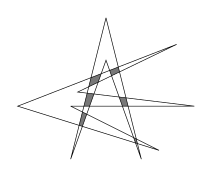
\includegraphics[width=6.4cm]{figures/2017-8-3B}
\end{center}

\itC Данная задача является обобщением \hyperref[float-ptb]{пункта B}. Из совершенно аналогичных соображений получаем ответ~--- от 3 до $m \cdot n$ углов.

\end{itemize}
